\documentclass[11pt,twoside,a4paper]{article}
\usepackage{fullpage}
\usepackage{graphicx}
\usepackage{amsmath}
\title{Wettbewerb Matrixoptik}
\author{Alain}

\begin{document}
	\maketitle
	\section{Analyse Aufgabenstellung}
	Ziel der Aufgabe ist, ein Optisches System aus vier bi-konvexen Linsen zu analysieren und mit Hilfe der Matrixoptik zu berechnen. \\
	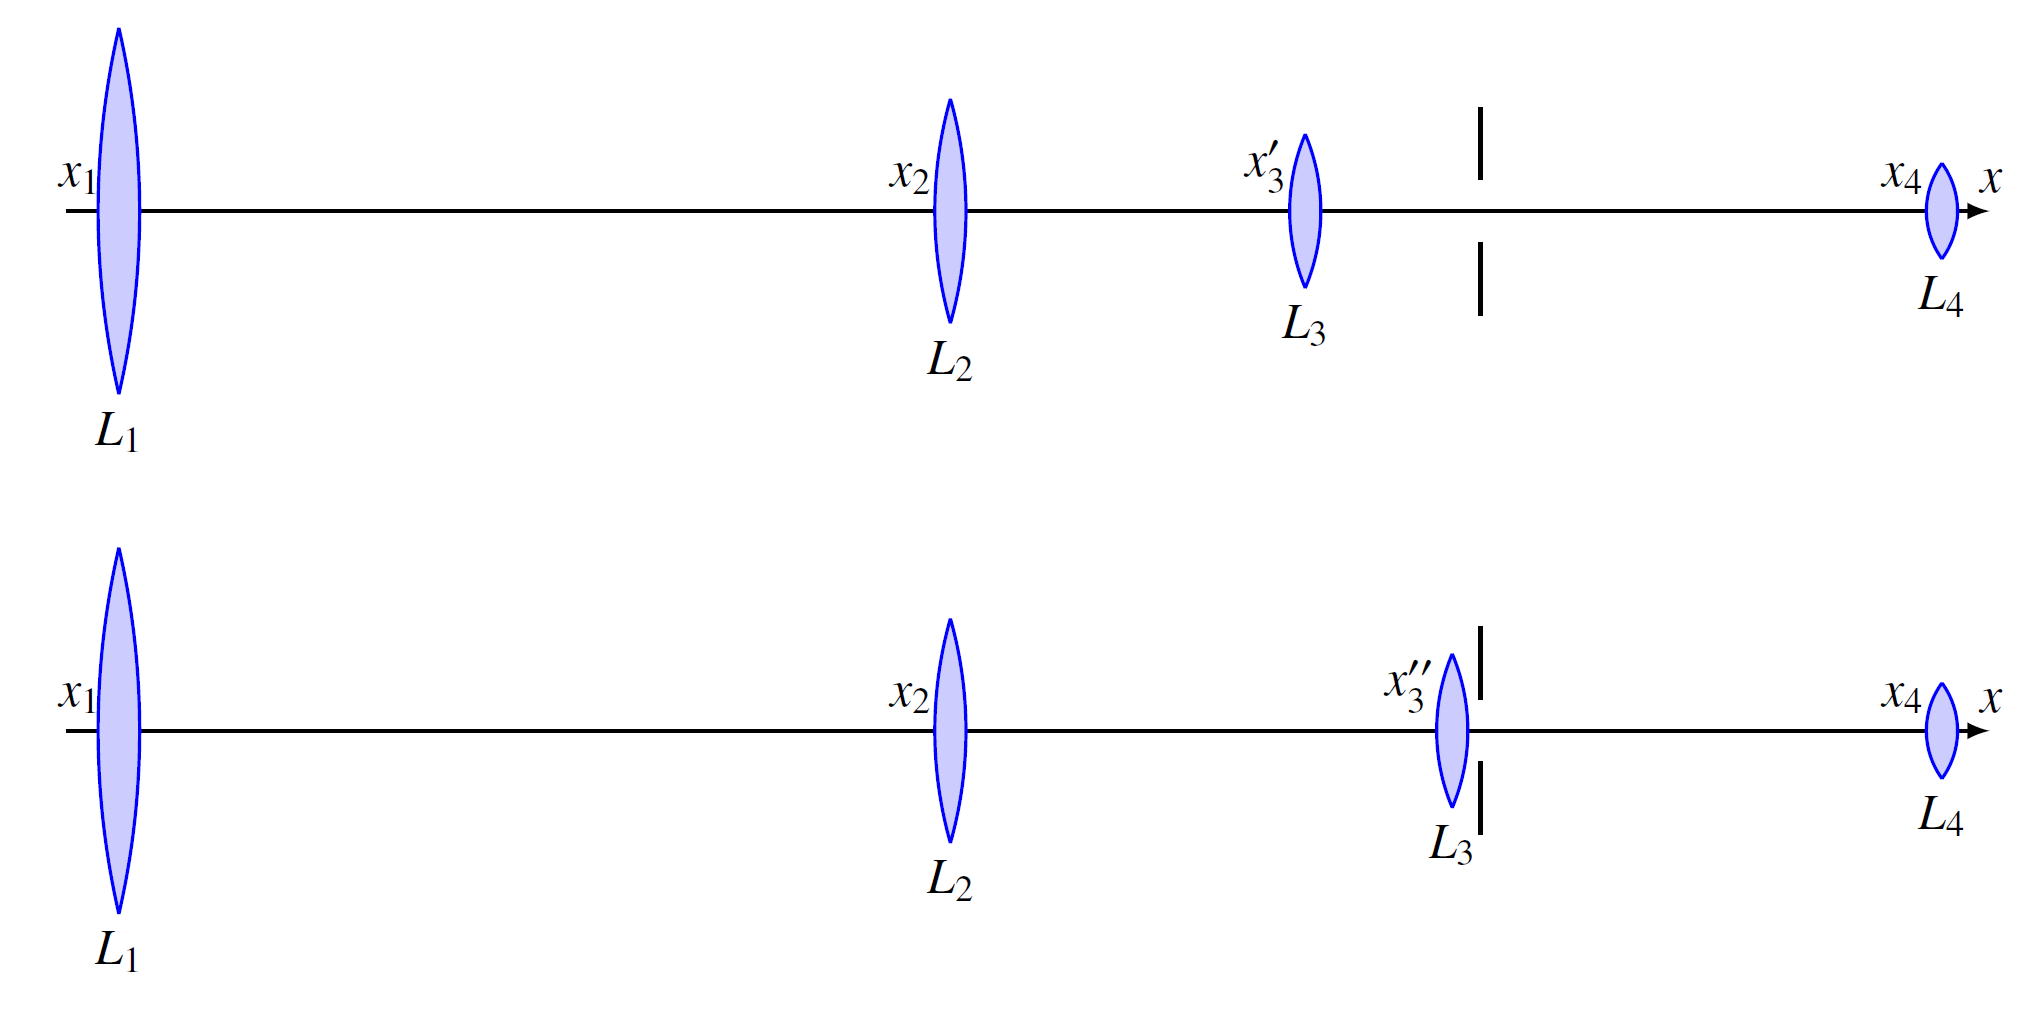
\includegraphics[scale=.25]{./system.PNG}
	\begin{table}
		\centering
		\begin{tabular}{lllll}
			Brechungsindex & Linse & Krümmungsradius R [mm]& Dicke [mm] & Position [mm] \\
			1.5 & \(x_{1}\) & 78.672364 & 4 & 0 \\
			1.5 & \(x_{2}\) & 39.603940 & 3 & 80 \\
			1.5 & \(x'_{3}\) & 19.013503 & 3 & \(x_{2} + 20 * (1+\frac{1}{\sqrt{2}})\)  \\
			1.5 & \(x''_{3}\) & 19.013503 & 3 & \(x_{2} + 20 * (1+\sqrt{2})\) \\
			1.5 & \(x_{4}\) & 7.8042263 & 3 & Unbekannt \\
		\end{tabular}
	\end{table} \\
	Das ganze Optische System, wie in der Darstellung dargestellt, mit den Daten der Tabelle 1 lässt sich mit Hilfe der Matrixoptik berechnen. Das Verhalten eines Lichtstrahles, welcher durch dieses Optische System geht, lässt sich mit einer Transfermatrix beschreiben. Durch diese Matrix lässt sich der Ausgangswinkel und -Höhe eines einfallenden Lichtstrahles mit bekanntem Einfallswinkel, und -Höhe berechnen.  
	\begin{equation} \label{Transfermatrix1}
	\begin{pmatrix}
	A & B \\
	C & D
	\end{pmatrix}
	\quad
	\begin{pmatrix}
	x_{1}\\
	\theta_{1}
	\end{pmatrix}
	\quad
	=
	\quad
	\begin{pmatrix}
	x_{2}\\
	\theta_{2}
	\end{pmatrix}
	\end{equation}
	\ref{Transfermatrix1} Beispiel einer Transfermatrix wobei x die vertikale Position des Lichtstrahles und \(\theta\) den Winkel beschreibt \\
	
	Das Ziel ist es eine solche Transfermatrix dieses optischen Systems zu berechnen. 
	\newpage 
	\section{Aufgabe 1}
\end{document}